%% Преамбула TeX-файла

% 1. Стиль и язык
\documentclass[utf8x, 14pt]{G7-32} % Стиль (по умолчанию будет 14pt)

% Остальные стандартные настройки убраны в preamble.inc.tex.
\sloppy

% Настройки стиля ГОСТ 7-32
% Для начала определяем, хотим мы или нет, чтобы рисунки и таблицы нумеровались в пределах раздела, или нам нужна сквозная нумерация.
\EqInChapter % формулы будут нумероваться в пределах раздела
\TableInChapter % таблицы будут нумероваться в пределах раздела
\PicInChapter % рисунки будут нумероваться в пределах раздела

% Добавляем гипертекстовое оглавление в PDF
\usepackage[
bookmarks=true, colorlinks=true, unicode=true,
urlcolor=black,linkcolor=black, anchorcolor=black,
citecolor=black, menucolor=black, filecolor=black,
]{hyperref}
\usepackage{pgfplots}
\usepackage{nomencl}

\usepackage{float}

\AfterHyperrefFix

\usepackage{microtype}% полезный пакет для микротипографии, увы под xelatex мало чего умеет, но под pdflatex хорошо улучшает читаемость

% Тире могут быть невидимы в Adobe Reader
\ifInvisibleDashes
\MakeDashesBold
\fi

\usepackage{graphicx}   % Пакет для включения рисунков

% С такими оно полями оно работает по-умолчанию:
% \RequirePackage[left=20mm,right=10mm,top=20mm,bottom=20mm,headsep=0pt,includefoot]{geometry}
% Если вас тошнит от поля в 10мм --- увеличивайте до 20-ти, ну и про переплёт не забывайте:
\geometry{right=10mm}
\geometry{left=30mm}
\geometry{bottom=20mm}
\geometry{ignorefoot}% считать от нижней границы текста


% Пакет Tikz
\usepackage{tikz}
\usetikzlibrary{arrows,positioning,shadows}

% Произвольная нумерация списков.
\usepackage{enumerate}

% ячейки в несколько строчек
\usepackage{multirow}

% itemize внутри tabular
\usepackage{paralist,array}

%\setlength{\parskip}{1ex plus0.5ex minus0.5ex} % разрыв между абзацами
\setlength{\parskip}{1ex} % разрыв между абзацами
\usepackage{blindtext}

% Центрирование подписей к плавающим окружениям
%\usepackage[justification=centering]{caption}

\usepackage{newfloat}
\DeclareFloatingEnvironment[
placement={!ht},
name=Equation
]{eqndescNoIndent}
\edef\fixEqndesc{\noexpand\setlength{\noexpand\parindent}{\the\parindent}\noexpand\setlength{\noexpand\parskip}{\the\parskip}}
\newenvironment{eqndesc}[1][!ht]{%
    \begin{eqndescNoIndent}[#1]%
\fixEqndesc%
}
{\end{eqndescNoIndent}}

\usepackage{afterpage}

\newcommand\blankpage{
	\null
	\thispagestyle{empty}
	\newpage
}



% Настройки листингов.
\ifPDFTeX
% 8 Листинги

\usepackage{listings}

% Значения по умолчанию
\lstset{
  basicstyle= \footnotesize,
  breakatwhitespace=true,% разрыв строк только на whitespacce
  breaklines=true,       % переносить длинные строки
%  captionpos=b,          % подписи снизу -- вроде не надо
  inputencoding=utf8x,
  numbers=left,          % нумерация слева
  numberstyle=\footnotesize,
  showspaces=false,      % показывать пробелы подчеркиваниями -- идиотизм 70-х годов
  showstringspaces=false,
  showtabs=false,        % и табы тоже
  stepnumber=1,
  tabsize=4,              % кому нужны табы по 8 символов?
  frame=single,
  xleftmargin=2.4em,
  framexleftmargin=2em
}

% Стиль для псевдокода: строчки обычно короткие, поэтому размер шрифта побольше
\lstdefinestyle{pseudocode}{
  basicstyle=\small,
  keywordstyle=\color{black}\bfseries\underbar,
  language=Pseudocode,
  numberstyle=\footnotesize,
  commentstyle=\footnotesize\it
}

% Стиль для обычного кода: маленький шрифт
\lstdefinestyle{realcode}{
  basicstyle=\scriptsize,
  numberstyle=\footnotesize
}

% Стиль для коротких кусков обычного кода: средний шрифт
\lstdefinestyle{simplecode}{
  basicstyle=\footnotesize,
  numberstyle=\footnotesize
}

% Стиль для BNF
\lstdefinestyle{grammar}{
  basicstyle=\footnotesize,
  numberstyle=\footnotesize,
  stringstyle=\bfseries\ttfamily,
  language=BNF
}

% Определим свой язык для написания псевдокодов на основе Python
\lstdefinelanguage[]{Pseudocode}[]{Python}{
  morekeywords={each,empty,wait,do},% ключевые слова добавлять сюда
  morecomment=[s]{\{}{\}},% комменты {а-ля Pascal} смотрятся нагляднее
  literate=% а сюда добавлять операторы, которые хотите отображать как мат. символы
    {->}{\ensuremath{$\rightarrow$}~}2%
    {<-}{\ensuremath{$\leftarrow$}~}2%
    {:=}{\ensuremath{$\leftarrow$}~}2%
    {<--}{\ensuremath{$\Longleftarrow$}~}2%
}[keywords,comments]

% Свой язык для задания грамматик в BNF
\lstdefinelanguage[]{BNF}[]{}{
  morekeywords={},
  morecomment=[s]{@}{@},
  morestring=[b]",%
  literate=%
    {->}{\ensuremath{$\rightarrow$}~}2%
    {*}{\ensuremath{$^*$}~}2%
    {+}{\ensuremath{$^+$}~}2%
    {|}{\ensuremath{$|$}~}2%
}[keywords,comments,strings]

% Подписи к листингам на русском языке.
\renewcommand\lstlistingname{Листинг}
\renewcommand\lstlistlistingname{Листинги}

\else
\usepackage{local-minted}
\fi

% Полезные макросы листингов.
% Любимые команды
\newcommand{\Code}[1]{\textbf{#1}}


% Стиль титульного листа и заголовки
\include{00-title}

\usepackage{csvsimple}
\usepackage{pgfplotstable}
\usepackage{datatool}

\begin{document}

\frontmatter % выключает нумерацию ВСЕГО; здесь начинаются ненумерованные главы: реферат, введение, глоссарий, сокращения и прочее.

\afterpage{\blankpage}
% пропущены страницы под тз и план (у меня их 2 тз и 1 план, итого 3, вам надо пропустить столько, сколько страниц у вас в тз и плане)


%\listoffigures                         % Список рисунков

%\listoftables                          % Список таблиц

%\NormRefs % Нормативные ссылки 
% Команды \breakingbeforechapters и \nonbreakingbeforechapters
% управляют разрывом страницы перед главами.
% По-умолчанию страница разрывается.

% \include{00-abstract}
% \nobreakingbeforechapters
% \breakingbeforechapters

\tableofcontents

% \printnomenclature % Автоматический список сокращений

%\Introduction
Цель работы: провести сравнительный анализ метода полного перебора и эвристического метода на базе муравьиного алгоритма.\\
При выполнении лабораторной работы поставлены такие задачи:
\begin{enumerate}[1)]
	\item реализовать метод полного перебора и метод на базе муравьиного алгоритма для решения задачи коммивояжёра с возвращением последнего в город, с которого он начал обход;
	\item провести параметризацию второго метода для выбранного класса задач;
	\item сделать выводы о результатах параметризации.
\end{enumerate}

%\mainmatter % это включает нумерацию глав и секций в документе ниже

\chapter{Аналитический раздел}
\label{cha:analysis}
В данном разделе будет представлено понятие задачи коммивояжера, рассмотрены алгоритм полного перебора и муравьиный алгоритм как способы ее решения.

\section{Задача коммивояжёра}
\label{sec:salesman}
Цель задачи коммивояжёра заключается в нахождении самого выгодного маршрута (кратчайшего, самого быстрого, наиболее дешевого), проходящего через все заданные точки (пункты, города) по одному разу, с последующим возвратом в исходную точку \cite{salesman}.
\par Условия задачи должны содержать критерий выгодности маршрута (т. е. должен ли он быть максимально коротким, быстрым, дешевым или все вместе), а также исходные данные в виде матрицы затрат (расстояния, стоимости, времени и т. д.) при перемещении между рассматриваемыми пунктами. 
\par Особенности задачи в том, что она довольно просто формулируется и найти хорошие решения для нее также относительно просто, но вместе с тем поиск действительно оптимального маршрута для большого набора данных - непростой и ресурсоемкий процесс. 
\par Для решения задачи коммивояжера ее надо представить как математическую модель. При этом исходные условия можно записать в формате матрицы - таблицы, где строкам соответсвуют города отправления, столбцам - города прибытия, а в ячейках указываются расстояния (время, стоимость) между ними; или в виде графа - схемы, состоящей из вершин, которые символизируют города, и соединяющих их ребер, длина которых соответствует расстоянию между городами.

\section{Методы ее решения}
\label{sec:methods}
Полный перебор - заключается в последовательном рассмотрении всех возможных маршрутов и выборе самого оптимального из них. Он является самым простым методом, который при этом всегда даёт верный ответ.
\par Идея муравьиного алгоритма -- моделирование поведения муравьёв, связанное с их способностью быстро находить кратчайший путь от муравейника к источнику пищи и адаптироваться к изменяющимся условиям, находя новый кратчайший путь. При своём движении муравей метит свой путь феромоном, и эта информация используется другими муравьями для выбора пути\cite{ulyanov}. 
\par Моделирование муравьёв связано с распределением феромона на тропе -- ребре графа в задаче коммивояжёра. При этом вероятность включения ребра в маршрут отдельного муравья пропорциональна количеству феромона.

\section{Муравьиные алгоритмы}
\label{sec:ants}
Для решения задачи коммивояжера можно описать  локальные правила поведения муравьев при выборе пути.
\begin{itemize}
	\item Муравьи имеют собственную <<память>>. Поскольку каждый город может быть посещен только 1 раз, у каждого муравья есть список уже посещенных городов -- список запретов. Обозначим через $J_{i,k}$ список городов, которые необходимо посетить муравью $k$, находящемся в городе i;
	\item муравьи обладают <<зрением>>  -- видимость есть эвристическое желание посетить город $j$, если муравей находится в городе i. Будем считать что видимость обратно пропорциональна расстоянию между городами $i$ и $j$ -- $D_{ij}$
	\begin{equation}
		\eta_{ij}=1/D_{ij}
	\end{equation}
	\item муравьи обладают <<обонянием>> -- они могут улавливать след феромона, подтверждающий желание посетить город j из города i, на основании опыта других муравьёв. Количество феромона на ребре $(i,j)$ в момент времени t обозначим через $\tau_{ij}(t)$.
\end{itemize}
\par Таким образом вероятностно-пропорциональное правило, определяющее вероятность перехода k-ого муравья из города i в город j:
\begin{equation}
	\begin{cases}
		P_{ij,k}(t)=\frac{[\tau_{ij}(t)]^{\alpha}*[\eta_{ij}]^{\beta}}{\sum\limits_{l\in J_{i,k}}[\tau_{ij}(t)]^{\alpha}*[\eta_{ij}}],\: j\in J_{i,k}\\
		P_{ij,k}=0, \: j \notin J_{i,k}
	\end{cases}
\end{equation}
где $\alpha, \beta$ -- параметры, задающие веса следа феромона, при $\alpha =0$ алгоритм вырождается до жадного.
\par Пройдя ребро $(i,j)$ муравей откладывает на нем некоторое количество феромона, которое должно быть связано с оптимальностью сделанного выбора. Пусть $T_{k}(t)$ есть маршрут, пройденный муравьём $k$ к моменту времени $t$, а $L_{k}(t)$ -- длина этого маршрута. Пусть также Q -- параметр, имеющий значение порядка длины оптимального пути. Тогда откладываемое количество феромона может быть задано в виде
\begin{equation}
	\delta\tau_{ij,k}(t)=\begin{cases}
		\frac{Q}{L_{k}(t)},\: (i,j)\in T_{k}(t);\\
		0, \: (i,j)\notin T_{k}(t).
	\end{cases}
\end{equation}
Правила внешней среды определяют, в первую очередь, испарение феромона. Пусть $p \in [0,1]$ есть коеффициент испарения, тогда правильно испарения имеет вид
\begin{equation}
	\tau_{ij}(t+1)=(1-p)*\tau_{ij}(t)+\delta\tau_{ij}(t);\quad \delta\tau_{ij}(t)=\sum\limits_{k=1}^{m}\delta\tau_{ij,k}(t)
\end{equation}
где m -- количество муравьев в колонии.
\section{Вывод}
\label{sec:res}
В данном разделе была представлена задача коммивояжёра, рассмотрены методы ее решения.
%\chapter{Конструкторский раздел}
\label{cha:design}
\textbf{Требования к вводу:}
\begin{enumerate}[1)]
	\item на вход подаются 2 строки;
	\item прописные и строчные буквы считаются разными символами.
\end{enumerate}
\textbf{Требования к программе:} две пустые строки являются корректным вводом.
\section{Схемы алгоритмов}
На рисунках 2.1-2.4 представлены схемы алгоритмов поиска расстояния Левенштейна и Дамерау-Левенштейна.\\
\label{sec:schemes}
\begin{figure}[H]
	\centering
	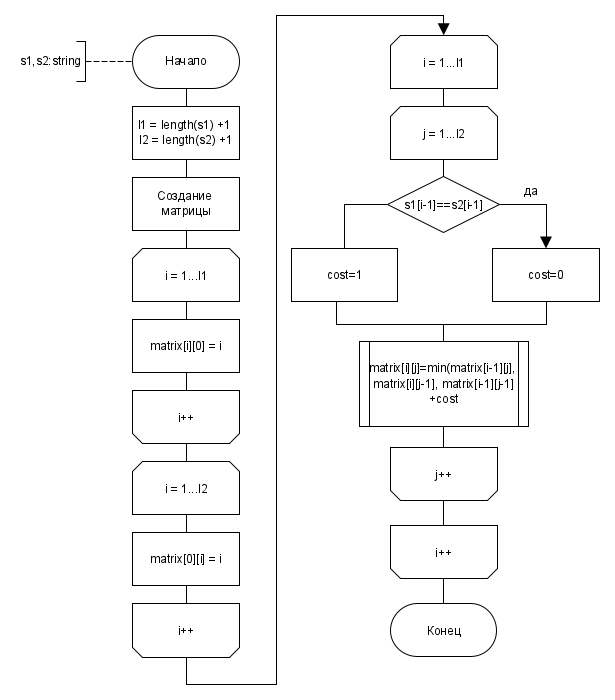
\includegraphics[width=0.6\linewidth]{src/Levenstein_m}
	\caption{Схема матричного алгоритма поиска расстояния Левенштейна}
	\label{fig:levensteinm}
\end{figure}
\begin{figure}[H]
	\centering
	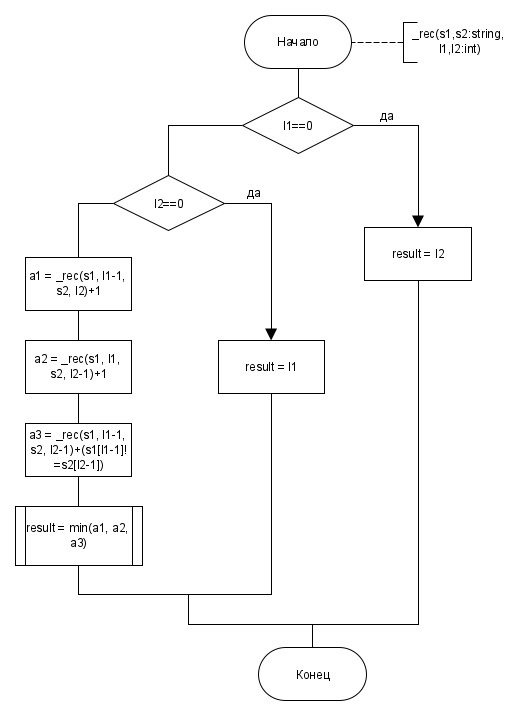
\includegraphics[width=0.7\linewidth]{src/Levenstein_r}
	\caption{Схема рекурсивного алгоритма поиска расстояния Левенштейна}
	\label{fig:levensteinr}
\end{figure}
\begin{figure}
	\centering
	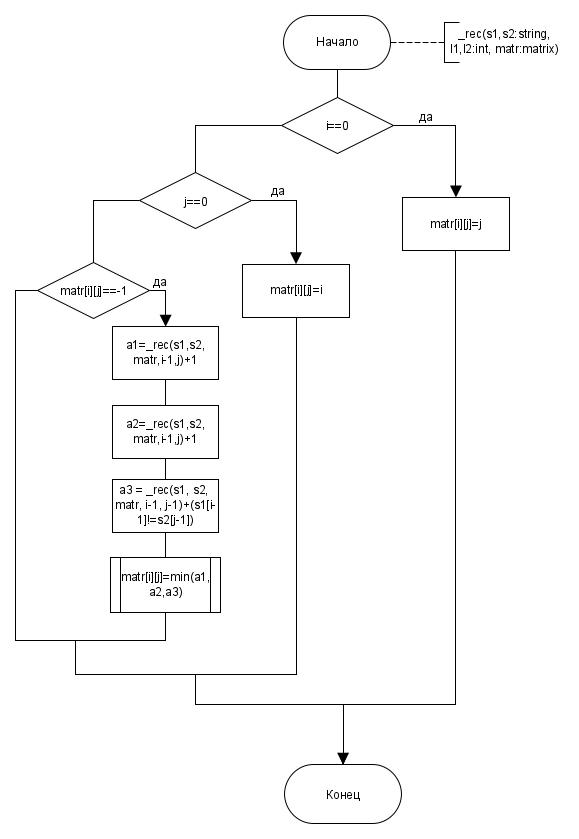
\includegraphics[width=0.8\linewidth]{src/Levenstein_rm}
	\caption{Схема матрично-рекурсивного алгоритма поиска расстояния Левенштейна}
	\label{fig:levensteinrm}
\end{figure}
Отличием матрично-рекурсивного алгоритма поиска расстояния Левенштейна от рекурсивного является сохранение результатов в матрицу, благодаря чему нет необходимости повторно пересчитывать значения функций.
\begin{figure}
	\centering
	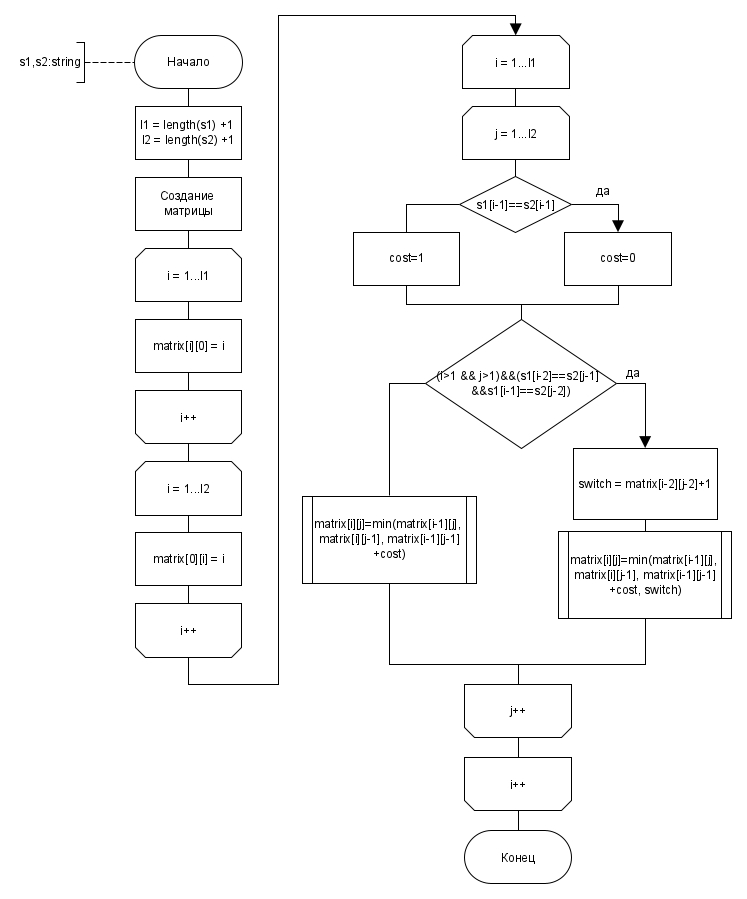
\includegraphics[width=0.8\linewidth]{src/Damerau_m}
	\caption{Схема матричного алгоритма поиска расстояния Дамерау-Левенштейна}
	\label{fig:dameraum}
\end{figure}

%\chapter{Технологический раздел}
\label{cha:impl}
В данном разделе будут представлены листинги кода реализованных алгоритмов.
\section{Средства реализации}
В данной работе используется язык программирования С++. Среда разработки Visual Studio Code. Для замера процессорного времени используется функция QueryPerformanceCounter из библиотеки windows.h.
\section{Листинг кода}
В листингах 3.1--3.3 приведены коды алгоритмов сортировки пузырьком с флагом, сортировки выбором и пирамидальной.
\begin{lstlisting}[caption= Сортировка пузырьком с флагом]
void bubbleSort(array_t array)
{
	bool changed = false;
	for (int i = 1; i < array.length; i++)
	{
		for (int j = 0; j < array.length - i; j++)
			if (array.array[j + 1] < array.array[j])
			{
				const int temp = array.array[j];
				array.array[j] = array.array[j + 1];
				array.array[j + 1] = temp;
				changed = true;
			}
		if (!changed)
			break;
	}
}
\end{lstlisting}

\begin{lstlisting}[caption= Сортировка выбором]
void selectionSort(array_t array)
{
	for(int i=0; i<array.length-1; i++)
	{
		int min_i = i;
		for(int j=i+1;j<array.length;j++)
		{
			if (array.array[j] < array.array[min_i])
			min_i = j;
		}
		if (min_i != i)
		{
			int tmp = array.array[i];
			array.array[i] = array.array[min_i];
			array.array[min_i] = tmp;
		}        
	}
}
\end{lstlisting}

\begin{lstlisting}[caption= Пирамидальная сортировка и необходимая для её работы функция siftDown]
void siftDown(array_t array, int i)
{
	int nMax = i;
	int value = array.array[i];
	while (true)
	{
		i = nMax;
		int childN = i*2 + 1;
		if ((childN < array.length) && (array.array[childN] > value))
			nMax = childN;
		childN++;
		if ((childN < array.length) && (array.array[childN] > array.array[nMax]))
			nMax = childN;
		if (nMax == i)
			break;
		array.array[i] = array.array[nMax];
		array.array[nMax] = value;
	}
}

void heapSort(array_t array)
{
	for (int i = array.length / 2 -1; i >= 0; --i)
		siftDown(array, i);
	while (array.length > 1)
	{
		array.length--;
		
		int firstElement = array.array[0];
		array.array[0] = array.array[array.length];
		array.array[array.length] = firstElement;
		
		siftDown(array, 0);
	}
}
\end{lstlisting}

\section{Проведение тестирования}
\label{sec:tests}
Изначально было проведено тестирование алгоритма сортировки пузырьком на массивах: [1,2,1,1,1], [5,4,3,2,1], [1,2,3,4,5], [5,1,2,4,3], все тесты были пройдены успешно.
\par После чего была проведена серия тестов на массивах длиной от 1 до 10. Сначала выполнялась сортировка пузырьковым алгоритмом, результат которого принимался за контрольное значение, после чего результаты сортировки алгоритмом выбора и пирамидальной сортировки сравнивались с контрольным значением и при совпадении результат считался корректным. Массивы заполнялись случайным образом и в возрастающем порядке. Все тесты были пройдены успешно.
%%%% mode: latex
%%%% TeX-master: "rpz"
%%%% End:

%\chapter{Исследовательский раздел}
\label{cha:research}
В данном разделе будет измерено время работы алгоритмов и сделаны выводы на основе полученных данных.
\section{Сравнительный анализ на основе замеров времени работы алгоритмов}
Для каждого из алгоритмов был проведён замер времени на массивах длиной от 5 до 50000 тысяч, с шагом 5000, для каждой длины были проведены измерения на массивах, отсортированных в убывающем, возрастающем порядках и заполненных случайными элементами. Для каждого теста было проведено 10 замеров, на графиках представлен усреднённый результат.
\par На рисунке 4.1 представлено сравнение времени работы алгоритмов при случайно заполненных массивах. На рисунках 4.1--4.3 время, обозначаемое t представлено в миллисекундах.
\begin{figure}[H]
\centering
\begin{tikzpicture}[scale=1.5]
\begin{axis}[
axis lines = left,
xlabel = {Длина массива},
ylabel = {$t$},
legend pos=north west,
ymajorgrids=true,
clip=false
]
\addplot[color=red, mark=square] table[x index=0, y index= 1] {src/tempRes/boubbleSortRandom.txt}; 
\addplot[color=green, mark=square] table[x index=0, y index= 1] {src/tempRes/selectionSortRandom.txt}; 
\addplot[color=blue, mark=square] table[x index=0, y index= 1] {src/tempRes/heapSortRandom.txt}; 

\addlegendentry{Пузырьком с флагом}
\addlegendentry{Выбором}
\addlegendentry{Пирамидальная}
\end{axis}
\end{tikzpicture}
\caption{Сравнение времени работы алгоритмов при случайно заполненных массивах}
\end{figure}

\par На рисунке 4.2 представлено сравнение времени работы алгоритмов при массивах, заполненных в возрастающем порядке.
\begin{figure}[H]
	\centering
	\begin{tikzpicture}[scale=1.5]
	\begin{axis}[
	axis lines = left,
	xlabel = {Длина массива},
	ylabel = {$t$},
	legend pos=north west,
	ymajorgrids=true
	]
	\addplot[color=red, mark=square] table[x index=0, y index= 1] {src/tempRes/boubbleSortSortedA.txt}; 
	\addplot[color=green, mark=square] table[x index=0, y index= 1] {src/tempRes/selectionSortSortedA.txt}; 
	\addplot[color=blue, mark=square] table[x index=0, y index= 1] {src/tempRes/heapSortSortedA.txt}; 
	
	\addlegendentry{Пузырьком с флагом}
	\addlegendentry{Выбором}
	\addlegendentry{Пирамидальная}
	\end{axis}
	\end{tikzpicture}
	\caption{Сравнение времени работы алгоритмов при массивах отсортированных в возрастающем порядке}
\end{figure}

\par На рисунке 4.3 представлено сравнение времени работы алгоритмов при массивах, заполненных в убывающем порядке.
\begin{figure}[H]
	\centering
	\begin{tikzpicture}[scale=1.5]
	\begin{axis}[
	axis lines = left,
	xlabel = {Длина массива},
	ylabel = {$t$},
	legend pos=north west,
	ymajorgrids=true
	]
	\addplot[color=red, mark=square] table[x index=0, y index= 1] {src/tempRes/boubbleSortSortedD.txt}; 
	\addplot[color=green, mark=square] table[x index=0, y index= 1] {src/tempRes/selectionSortSortedD.txt}; 
	\addplot[color=blue, mark=square] table[x index=0, y index= 1] {src/tempRes/heapSortSortedD.txt}; 
	
	\addlegendentry{Пузырьком с флагом}
	\addlegendentry{Выбором}
	\addlegendentry{Пирамидальная}
	\end{axis}
	\end{tikzpicture}
	\caption{Сравнение времени работы алгоритмов при массивах отсортированных в убывающем порядке}
\end{figure}

\par Из рисунков 4.1--4.3 видно, что наиболее эффективным по времени в случаях с случайно заполненными массивами и массивами, заполненными в убывающем порядке оказался алгоритм пирамидальной сортировки, в то время как сортировка пузырьком с флагом самая быстрая при массивах, отсортированных в возрастающем порядке.
\par Таким образом, данные, полученные в результате проведённых экспериментов подтверждают корректность рассчитанных ранее трудоёмкостей алгоритмов.
\par\textbf{Вывод} 
\par В итоге, можно сказать о том, что пирамидальная сортировка является наиболее эффективной по времени среди рассмотренных алгоритмов.


\backmatter %% Здесь заканчивается нумерованная часть документа и начинаются ссылки и
            
%\Conclusion % заключение к отчёту
В результате лабораторной работы цель была достигнута -- были изучены алгоритмы умножения матриц. Все поставленные задачи были выполнены: оптимизирован алгоритм Винограда, дана теоретическая оценка трудоёмкости стандартного алгоритма, алгоритма Винограда и улучшенного алгоритма Винограда, все они были реализованы и проведён их сравнительный анализ.%% заключение


%% % Список литературы при помощи BibTeX
% Юзать так:
%
% pdflatex rpz
% bibtex rpz
% pdflatex rpz

\bibliographystyle{ugost2008}
\bibliography{rpz}

%%% Local Variables: 
%%% mode: latex
%%% TeX-master: "rpz"
%%% End: 


%
%\appendix   % Тут идут приложения
%\chapter{}
	\begin{longtable}{|l|l|l|l|l|l|l|}
		\caption{Результат параметризации}\label{ap:t}\\
		\hline
		$\alpha$ & p   & tmax & d1 & d2 & dr1 & dr2 \\ \hline
		0     & 0.1 & 10   & 60 & 57 & -2  & -2  \\ \hline
		0     & 0.1 & 20   & 62 & 58 & -4  & -3  \\ \hline
		0     & 0.1 & 30   & 61 & 58 & -3  & -3  \\ \hline
		0     & 0.1 & 40   & 61 & 59 & -3  & -4  \\ \hline
		0     & 0.1 & 50   & 61 & 57 & -3  & -2  \\ \hline
		0     & 0.3 & 10   & 62 & 59 & -4  & -4  \\ \hline
		0     & 0.3 & 20   & 62 & 58 & -4  & -3  \\ \hline
		0     & 0.3 & 30   & 60 & 58 & -2  & -3  \\ \hline
		0     & 0.3 & 40   & 61 & 57 & -3  & -2  \\ \hline
		0     & 0.3 & 50   & 60 & 58 & -2  & -3  \\ \hline
		0     & 0.5 & 10   & 61 & 59 & -3  & -4  \\ \hline
		0     & 0.5 & 20   & 62 & 57 & -4  & -2  \\ \hline
		0     & 0.5 & 30   & 61 & 58 & -3  & -3  \\ \hline
		0     & 0.5 & 40   & 59 & 59 & -1  & -4  \\ \hline
		0     & 0.5 & 50   & 60 & 57 & -2  & -2  \\ \hline
		0     & 0.7 & 10   & 60 & 59 & -2  & -4  \\ \hline
		0     & 0.7 & 20   & 62 & 58 & -4  & -3  \\ \hline
		0     & 0.7 & 30   & 60 & 58 & -2  & -3  \\ \hline
		0     & 0.7 & 40   & 62 & 57 & -4  & -2  \\ \hline
		0     & 0.7 & 50   & 60 & 58 & -2  & -3  \\ \hline
		0     & 0.9 & 10   & 61 & 59 & -3  & -4  \\ \hline
		0     & 0.9 & 20   & 61 & 57 & -3  & -2  \\ \hline
		0     & 0.9 & 30   & 61 & 56 & -3  & -1  \\ \hline
		0     & 0.9 & 40   & 61 & 58 & -3  & -3  \\ \hline
		0     & 0.9 & 50   & 60 & 58 & -2  & -3  \\ \hline
		0     & 0.1 & 10   & 59 & 56 & -1  & -1  \\ \hline
		0     & 0.1 & 20   & 59 & 57 & -1  & -2  \\ \hline
		0     & 0.1 & 30   & 59 & 56 & -1  & -1  \\ \hline
		0     & 0.1 & 40   & 59 & 56 & -1  & -1  \\ \hline
		0     & 0.1 & 50   & 59 & 57 & -1  & -2  \\ \hline
		0     & 0.3 & 10   & 60 & 57 & -2  & -2  \\ \hline
		0     & 0.3 & 20   & 60 & 56 & -2  & -1  \\ \hline
		0     & 0.3 & 30   & 60 & 55 & -2  & 0   \\ \hline
		0     & 0.3 & 40   & 59 & 56 & -1  & -1  \\ \hline
		0     & 0.3 & 50   & 59 & 57 & -1  & -2  \\ \hline
		0     & 0.5 & 10   & 59 & 57 & -1  & -2  \\ \hline
		0     & 0.5 & 20   & 59 & 57 & -1  & -2  \\ \hline
		0     & 0.5 & 30   & 59 & 56 & -1  & -1  \\ \hline
		0     & 0.5 & 40   & 58 & 56 & 0   & -1  \\ \hline
		0     & 0.5 & 50   & 58 & 56 & 0   & -1  \\ \hline
		0     & 0.7 & 10   & 59 & 57 & -1  & -2  \\ \hline
		0     & 0.7 & 20   & 60 & 56 & -2  & -1  \\ \hline
		0     & 0.7 & 30   & 58 & 57 & 0   & -2  \\ \hline
		0     & 0.7 & 40   & 59 & 55 & -1  & 0   \\ \hline
		0     & 0.7 & 50   & 59 & 56 & -1  & -1  \\ \hline
		0     & 0.9 & 10   & 60 & 56 & -2  & -1  \\ \hline
		0     & 0.9 & 20   & 60 & 57 & -2  & -2  \\ \hline
		0     & 0.9 & 30   & 58 & 56 & 0   & -1  \\ \hline
		0     & 0.9 & 40   & 59 & 56 & -1  & -1  \\ \hline
		0     & 0.9 & 50   & 58 & 55 & 0   & 0   \\ \hline
		0     & 0.1 & 10   & 59 & 55 & -1  & 0   \\ \hline
		0     & 0.1 & 20   & 59 & 55 & -1  & 0   \\ \hline
		0     & 0.1 & 30   & 59 & 56 & -1  & -1  \\ \hline
		0     & 0.1 & 40   & 59 & 56 & -1  & -1  \\ \hline
		0     & 0.1 & 50   & 58 & 55 & 0   & 0   \\ \hline
		0     & 0.3 & 10   & 59 & 56 & -1  & -1  \\ \hline
		0     & 0.3 & 20   & 58 & 56 & 0   & -1  \\ \hline
		0     & 0.3 & 30   & 58 & 56 & 0   & -1  \\ \hline
		0     & 0.3 & 40   & 58 & 55 & 0   & 0   \\ \hline
		0     & 0.3 & 50   & 58 & 55 & 0   & 0   \\ \hline
		0     & 0.5 & 10   & 59 & 55 & -1  & 0   \\ \hline
		0     & 0.5 & 20   & 59 & 56 & -1  & -1  \\ \hline
		0     & 0.5 & 30   & 58 & 56 & 0   & -1  \\ \hline
		0     & 0.5 & 40   & 59 & 56 & -1  & -1  \\ \hline
		0     & 0.5 & 50   & 59 & 56 & -1  & -1  \\ \hline
		0     & 0.7 & 10   & 58 & 57 & 0   & -2  \\ \hline
		0     & 0.7 & 20   & 59 & 56 & -1  & -1  \\ \hline
		0     & 0.7 & 30   & 58 & 56 & 0   & -1  \\ \hline
		0     & 0.7 & 40   & 58 & 56 & 0   & -1  \\ \hline
		0     & 0.7 & 50   & 58 & 55 & 0   & 0   \\ \hline
		0     & 0.9 & 10   & 60 & 56 & -2  & -1  \\ \hline
		0     & 0.9 & 20   & 59 & 55 & -1  & 0   \\ \hline
		0     & 0.9 & 30   & 58 & 56 & 0   & -1  \\ \hline
		0     & 0.9 & 40   & 58 & 55 & 0   & 0   \\ \hline
		0     & 0.9 & 50   & 58 & 55 & 0   & 0   \\ \hline
		0     & 0.1 & 10   & 58 & 56 & 0   & -1  \\ \hline
		0     & 0.1 & 20   & 58 & 56 & 0   & -1  \\ \hline
		0     & 0.1 & 30   & 58 & 56 & 0   & -1  \\ \hline
		0     & 0.1 & 40   & 58 & 55 & 0   & 0   \\ \hline
		0     & 0.1 & 50   & 58 & 55 & 0   & 0   \\ \hline
		0     & 0.3 & 10   & 59 & 55 & -1  & 0   \\ \hline
		0     & 0.3 & 20   & 58 & 55 & 0   & 0   \\ \hline
		0     & 0.3 & 30   & 58 & 55 & 0   & 0   \\ \hline
		0     & 0.3 & 40   & 58 & 55 & 0   & 0   \\ \hline
		0     & 0.3 & 50   & 58 & 55 & 0   & 0   \\ \hline
		0     & 0.5 & 10   & 59 & 56 & -1  & -1  \\ \hline
		0     & 0.5 & 20   & 58 & 55 & 0   & 0   \\ \hline
		0     & 0.5 & 30   & 58 & 55 & 0   & 0   \\ \hline
		0     & 0.5 & 40   & 58 & 55 & 0   & 0   \\ \hline
		0     & 0.5 & 50   & 58 & 55 & 0   & 0   \\ \hline
		0     & 0.7 & 10   & 58 & 55 & 0   & 0   \\ \hline
		0     & 0.7 & 20   & 58 & 55 & 0   & 0   \\ \hline
		0     & 0.7 & 30   & 58 & 55 & 0   & 0   \\ \hline
		0     & 0.7 & 40   & 58 & 55 & 0   & 0   \\ \hline
		0     & 0.7 & 50   & 58 & 55 & 0   & 0   \\ \hline
		0     & 0.9 & 10   & 58 & 56 & 0   & -1  \\ \hline
		0     & 0.9 & 20   & 58 & 55 & 0   & 0   \\ \hline
		0     & 0.9 & 30   & 59 & 55 & -1  & 0   \\ \hline
		0     & 0.9 & 40   & 58 & 55 & 0   & 0   \\ \hline
		0     & 0.9 & 50   & 58 & 55 & 0   & 0   \\ \hline
		0     & 0.1 & 10   & 58 & 55 & 0   & 0   \\ \hline
		0     & 0.1 & 20   & 58 & 55 & 0   & 0   \\ \hline
		0     & 0.1 & 30   & 58 & 55 & 0   & 0   \\ \hline
		0     & 0.1 & 40   & 58 & 55 & 0   & 0   \\ \hline
		0     & 0.1 & 50   & 58 & 55 & 0   & 0   \\ \hline
		0     & 0.3 & 10   & 58 & 55 & 0   & 0   \\ \hline
		0     & 0.3 & 20   & 58 & 55 & 0   & 0   \\ \hline
		0     & 0.3 & 30   & 58 & 55 & 0   & 0   \\ \hline
		0     & 0.3 & 40   & 58 & 55 & 0   & 0   \\ \hline
		0     & 0.3 & 50   & 58 & 55 & 0   & 0   \\ \hline
		0     & 0.5 & 10   & 58 & 55 & 0   & 0   \\ \hline
		0     & 0.5 & 20   & 58 & 55 & 0   & 0   \\ \hline
		0     & 0.5 & 30   & 58 & 55 & 0   & 0   \\ \hline
		0     & 0.5 & 40   & 58 & 55 & 0   & 0   \\ \hline
		0     & 0.5 & 50   & 58 & 55 & 0   & 0   \\ \hline
		0     & 0.7 & 10   & 58 & 55 & 0   & 0   \\ \hline
		0     & 0.7 & 20   & 59 & 56 & -1  & -1  \\ \hline
		0     & 0.7 & 30   & 58 & 55 & 0   & 0   \\ \hline
		0     & 0.7 & 40   & 58 & 55 & 0   & 0   \\ \hline
		0     & 0.7 & 50   & 58 & 55 & 0   & 0   \\ \hline
		0     & 0.9 & 10   & 58 & 55 & 0   & 0   \\ \hline
		0     & 0.9 & 20   & 58 & 55 & 0   & 0   \\ \hline
		0     & 0.9 & 30   & 58 & 55 & 0   & 0   \\ \hline
		0     & 0.9 & 40   & 58 & 55 & 0   & 0   \\ \hline
		0     & 0.9 & 50   & 58 & 55 & 0   & 0   \\ \hline
		2     & 0.1 & 10   & 62 & 59 & -4  & -4  \\ \hline
		2     & 0.1 & 20   & 60 & 58 & -2  & -3  \\ \hline
		2     & 0.1 & 30   & 60 & 57 & -2  & -2  \\ \hline
		2     & 0.1 & 40   & 60 & 57 & -2  & -2  \\ \hline
		2     & 0.1 & 50   & 59 & 57 & -1  & -2  \\ \hline
		2     & 0.3 & 10   & 62 & 60 & -4  & -5  \\ \hline
		2     & 0.3 & 20   & 59 & 60 & -1  & -5  \\ \hline
		2     & 0.3 & 30   & 60 & 58 & -2  & -3  \\ \hline
		2     & 0.3 & 40   & 60 & 61 & -2  & -6  \\ \hline
		2     & 0.3 & 50   & 60 & 57 & -2  & -2  \\ \hline
		2     & 0.5 & 10   & 61 & 59 & -3  & -4  \\ \hline
		2     & 0.5 & 20   & 60 & 57 & -2  & -2  \\ \hline
		2     & 0.5 & 30   & 61 & 58 & -3  & -3  \\ \hline
		2     & 0.5 & 40   & 60 & 56 & -2  & -1  \\ \hline
		2     & 0.5 & 50   & 60 & 58 & -2  & -3  \\ \hline
		2     & 0.7 & 10   & 60 & 59 & -2  & -4  \\ \hline
		2     & 0.7 & 20   & 61 & 58 & -3  & -3  \\ \hline
		2     & 0.7 & 30   & 60 & 56 & -2  & -1  \\ \hline
		2     & 0.7 & 40   & 61 & 58 & -3  & -3  \\ \hline
		2     & 0.7 & 50   & 61 & 57 & -3  & -2  \\ \hline
		2     & 0.9 & 10   & 61 & 58 & -3  & -3  \\ \hline
		2     & 0.9 & 20   & 61 & 56 & -3  & -1  \\ \hline
		2     & 0.9 & 30   & 60 & 57 & -2  & -2  \\ \hline
		2     & 0.9 & 40   & 60 & 56 & -2  & -1  \\ \hline
		2     & 0.9 & 50   & 59 & 57 & -1  & -2  \\ \hline
		2     & 0.1 & 10   & 59 & 57 & -1  & -2  \\ \hline
		2     & 0.1 & 20   & 59 & 56 & -1  & -1  \\ \hline
		2     & 0.1 & 30   & 59 & 55 & -1  & 0   \\ \hline
		2     & 0.1 & 40   & 58 & 57 & 0   & -2  \\ \hline
		2     & 0.1 & 50   & 59 & 55 & -1  & 0   \\ \hline
		2     & 0.3 & 10   & 61 & 57 & -3  & -2  \\ \hline
		2     & 0.3 & 20   & 59 & 57 & -1  & -2  \\ \hline
		2     & 0.3 & 30   & 60 & 56 & -2  & -1  \\ \hline
		2     & 0.3 & 40   & 58 & 55 & 0   & 0   \\ \hline
		2     & 0.3 & 50   & 59 & 56 & -1  & -1  \\ \hline
		2     & 0.5 & 10   & 60 & 57 & -2  & -2  \\ \hline
		2     & 0.5 & 20   & 58 & 56 & 0   & -1  \\ \hline
		2     & 0.5 & 30   & 60 & 56 & -2  & -1  \\ \hline
		2     & 0.5 & 40   & 59 & 57 & -1  & -2  \\ \hline
		2     & 0.5 & 50   & 60 & 56 & -2  & -1  \\ \hline
		2     & 0.7 & 10   & 60 & 57 & -2  & -2  \\ \hline
		2     & 0.7 & 20   & 59 & 57 & -1  & -2  \\ \hline
		2     & 0.7 & 30   & 59 & 56 & -1  & -1  \\ \hline
		2     & 0.7 & 40   & 59 & 56 & -1  & -1  \\ \hline
		2     & 0.7 & 50   & 59 & 56 & -1  & -1  \\ \hline
		2     & 0.9 & 10   & 61 & 58 & -3  & -3  \\ \hline
		2     & 0.9 & 20   & 59 & 56 & -1  & -1  \\ \hline
		2     & 0.9 & 30   & 60 & 56 & -2  & -1  \\ \hline
		2     & 0.9 & 40   & 59 & 56 & -1  & -1  \\ \hline
		2     & 0.9 & 50   & 59 & 56 & -1  & -1  \\ \hline
		2     & 0.1 & 10   & 60 & 55 & -2  & 0   \\ \hline
		2     & 0.1 & 20   & 59 & 55 & -1  & 0   \\ \hline
		2     & 0.1 & 30   & 59 & 55 & -1  & 0   \\ \hline
		2     & 0.1 & 40   & 58 & 55 & 0   & 0   \\ \hline
		2     & 0.1 & 50   & 58 & 55 & 0   & 0   \\ \hline
		2     & 0.3 & 10   & 59 & 57 & -1  & -2  \\ \hline
		2     & 0.3 & 20   & 59 & 55 & -1  & 0   \\ \hline
		2     & 0.3 & 30   & 58 & 56 & 0   & -1  \\ \hline
		2     & 0.3 & 40   & 58 & 56 & 0   & -1  \\ \hline
		2     & 0.3 & 50   & 59 & 55 & -1  & 0   \\ \hline
		2     & 0.5 & 10   & 58 & 55 & 0   & 0   \\ \hline
		2     & 0.5 & 20   & 58 & 55 & 0   & 0   \\ \hline
		2     & 0.5 & 30   & 59 & 55 & -1  & 0   \\ \hline
		2     & 0.5 & 40   & 58 & 55 & 0   & 0   \\ \hline
		2     & 0.5 & 50   & 58 & 55 & 0   & 0   \\ \hline
		2     & 0.7 & 10   & 58 & 56 & 0   & -1  \\ \hline
		2     & 0.7 & 20   & 59 & 56 & -1  & -1  \\ \hline
		2     & 0.7 & 30   & 59 & 55 & -1  & 0   \\ \hline
		2     & 0.7 & 40   & 58 & 55 & 0   & 0   \\ \hline
		2     & 0.7 & 50   & 58 & 55 & 0   & 0   \\ \hline
		2     & 0.9 & 10   & 58 & 55 & 0   & 0   \\ \hline
		2     & 0.9 & 20   & 58 & 56 & 0   & -1  \\ \hline
		2     & 0.9 & 30   & 59 & 56 & -1  & -1  \\ \hline
		2     & 0.9 & 40   & 59 & 55 & -1  & 0   \\ \hline
		2     & 0.9 & 50   & 59 & 55 & -1  & 0   \\ \hline
		2     & 0.1 & 10   & 59 & 55 & -1  & 0   \\ \hline
		2     & 0.1 & 20   & 58 & 56 & 0   & -1  \\ \hline
		2     & 0.1 & 30   & 58 & 55 & 0   & 0   \\ \hline
		2     & 0.1 & 40   & 58 & 55 & 0   & 0   \\ \hline
		2     & 0.1 & 50   & 58 & 55 & 0   & 0   \\ \hline
		2     & 0.3 & 10   & 59 & 55 & -1  & 0   \\ \hline
		2     & 0.3 & 20   & 58 & 55 & 0   & 0   \\ \hline
		2     & 0.3 & 30   & 58 & 55 & 0   & 0   \\ \hline
		2     & 0.3 & 40   & 58 & 55 & 0   & 0   \\ \hline
		2     & 0.3 & 50   & 58 & 55 & 0   & 0   \\ \hline
		2     & 0.5 & 10   & 59 & 55 & -1  & 0   \\ \hline
		2     & 0.5 & 20   & 58 & 55 & 0   & 0   \\ \hline
		2     & 0.5 & 30   & 58 & 55 & 0   & 0   \\ \hline
		2     & 0.5 & 40   & 58 & 55 & 0   & 0   \\ \hline
		2     & 0.5 & 50   & 58 & 55 & 0   & 0   \\ \hline
		2     & 0.7 & 10   & 58 & 56 & 0   & -1  \\ \hline
		2     & 0.7 & 20   & 58 & 55 & 0   & 0   \\ \hline
		2     & 0.7 & 30   & 58 & 55 & 0   & 0   \\ \hline
		2     & 0.7 & 40   & 58 & 55 & 0   & 0   \\ \hline
		2     & 0.7 & 50   & 58 & 55 & 0   & 0   \\ \hline
		2     & 0.9 & 10   & 59 & 55 & -1  & 0   \\ \hline
		2     & 0.9 & 20   & 58 & 55 & 0   & 0   \\ \hline
		2     & 0.9 & 30   & 58 & 55 & 0   & 0   \\ \hline
		2     & 0.9 & 40   & 58 & 55 & 0   & 0   \\ \hline
		2     & 0.9 & 50   & 58 & 55 & 0   & 0   \\ \hline
		2     & 0.1 & 10   & 58 & 56 & 0   & -1  \\ \hline
		2     & 0.1 & 20   & 58 & 55 & 0   & 0   \\ \hline
		2     & 0.1 & 30   & 58 & 55 & 0   & 0   \\ \hline
		2     & 0.1 & 40   & 58 & 55 & 0   & 0   \\ \hline
		2     & 0.1 & 50   & 58 & 55 & 0   & 0   \\ \hline
		2     & 0.3 & 10   & 58 & 55 & 0   & 0   \\ \hline
		2     & 0.3 & 20   & 58 & 55 & 0   & 0   \\ \hline
		2     & 0.3 & 30   & 58 & 55 & 0   & 0   \\ \hline
		2     & 0.3 & 40   & 58 & 55 & 0   & 0   \\ \hline
		2     & 0.3 & 50   & 58 & 55 & 0   & 0   \\ \hline
		2     & 0.5 & 10   & 59 & 55 & -1  & 0   \\ \hline
		2     & 0.5 & 20   & 58 & 55 & 0   & 0   \\ \hline
		2     & 0.5 & 30   & 58 & 55 & 0   & 0   \\ \hline
		2     & 0.5 & 40   & 58 & 55 & 0   & 0   \\ \hline
		2     & 0.5 & 50   & 58 & 55 & 0   & 0   \\ \hline
		2     & 0.7 & 10   & 58 & 55 & 0   & 0   \\ \hline
		2     & 0.7 & 20   & 58 & 55 & 0   & 0   \\ \hline
		2     & 0.7 & 30   & 58 & 55 & 0   & 0   \\ \hline
		2     & 0.7 & 40   & 58 & 55 & 0   & 0   \\ \hline
		2     & 0.7 & 50   & 58 & 55 & 0   & 0   \\ \hline
		2     & 0.9 & 10   & 58 & 55 & 0   & 0   \\ \hline
		2     & 0.9 & 20   & 58 & 55 & 0   & 0   \\ \hline
		2     & 0.9 & 30   & 58 & 55 & 0   & 0   \\ \hline
		2     & 0.9 & 40   & 58 & 55 & 0   & 0   \\ \hline
		2     & 0.9 & 50   & 58 & 55 & 0   & 0   \\ \hline
		4     & 0.1 & 10   & 61 & 60 & -3  & -5  \\ \hline
		4     & 0.1 & 20   & 61 & 59 & -3  & -4  \\ \hline
		4     & 0.1 & 30   & 59 & 57 & -1  & -2  \\ \hline
		4     & 0.1 & 40   & 60 & 57 & -2  & -2  \\ \hline
		4     & 0.1 & 50   & 60 & 55 & -2  & 0   \\ \hline
		4     & 0.3 & 10   & 62 & 58 & -4  & -3  \\ \hline
		4     & 0.3 & 20   & 61 & 57 & -3  & -2  \\ \hline
		4     & 0.3 & 30   & 61 & 58 & -3  & -3  \\ \hline
		4     & 0.3 & 40   & 60 & 58 & -2  & -3  \\ \hline
		4     & 0.3 & 50   & 61 & 58 & -3  & -3  \\ \hline
		4     & 0.5 & 10   & 61 & 60 & -3  & -5  \\ \hline
		4     & 0.5 & 20   & 60 & 58 & -2  & -3  \\ \hline
		4     & 0.5 & 30   & 61 & 58 & -3  & -3  \\ \hline
		4     & 0.5 & 40   & 60 & 58 & -2  & -3  \\ \hline
		4     & 0.5 & 50   & 60 & 58 & -2  & -3  \\ \hline
		4     & 0.7 & 10   & 60 & 59 & -2  & -4  \\ \hline
		4     & 0.7 & 20   & 60 & 56 & -2  & -1  \\ \hline
		4     & 0.7 & 30   & 61 & 57 & -3  & -2  \\ \hline
		4     & 0.7 & 40   & 61 & 58 & -3  & -3  \\ \hline
		4     & 0.7 & 50   & 60 & 57 & -2  & -2  \\ \hline
		4     & 0.9 & 10   & 63 & 60 & -5  & -5  \\ \hline
		4     & 0.9 & 20   & 60 & 59 & -2  & -4  \\ \hline
		4     & 0.9 & 30   & 61 & 58 & -3  & -3  \\ \hline
		4     & 0.9 & 40   & 60 & 59 & -2  & -4  \\ \hline
		4     & 0.9 & 50   & 61 & 57 & -3  & -2  \\ \hline
		4     & 0.1 & 10   & 61 & 56 & -3  & -1  \\ \hline
		4     & 0.1 & 20   & 59 & 58 & -1  & -3  \\ \hline
		4     & 0.1 & 30   & 59 & 57 & -1  & -2  \\ \hline
		4     & 0.1 & 40   & 60 & 55 & -2  & 0   \\ \hline
		4     & 0.1 & 50   & 59 & 56 & -1  & -1  \\ \hline
		4     & 0.3 & 10   & 58 & 57 & 0   & -2  \\ \hline
		4     & 0.3 & 20   & 59 & 56 & -1  & -1  \\ \hline
		4     & 0.3 & 30   & 60 & 57 & -2  & -2  \\ \hline
		4     & 0.3 & 40   & 58 & 56 & 0   & -1  \\ \hline
		4     & 0.3 & 50   & 59 & 55 & -1  & 0   \\ \hline
		4     & 0.5 & 10   & 61 & 56 & -3  & -1  \\ \hline
		4     & 0.5 & 20   & 58 & 56 & 0   & -1  \\ \hline
		4     & 0.5 & 30   & 60 & 57 & -2  & -2  \\ \hline
		4     & 0.5 & 40   & 59 & 55 & -1  & 0   \\ \hline
		4     & 0.5 & 50   & 59 & 56 & -1  & -1  \\ \hline
		4     & 0.7 & 10   & 60 & 57 & -2  & -2  \\ \hline
		4     & 0.7 & 20   & 59 & 55 & -1  & 0   \\ \hline
		4     & 0.7 & 30   & 59 & 56 & -1  & -1  \\ \hline
		4     & 0.7 & 40   & 60 & 56 & -2  & -1  \\ \hline
		4     & 0.7 & 50   & 60 & 56 & -2  & -1  \\ \hline
		4     & 0.9 & 10   & 60 & 56 & -2  & -1  \\ \hline
		4     & 0.9 & 20   & 59 & 55 & -1  & 0   \\ \hline
		4     & 0.9 & 30   & 58 & 55 & 0   & 0   \\ \hline
		4     & 0.9 & 40   & 59 & 55 & -1  & 0   \\ \hline
		4     & 0.9 & 50   & 58 & 56 & 0   & -1  \\ \hline
		4     & 0.1 & 10   & 60 & 56 & -2  & -1  \\ \hline
		4     & 0.1 & 20   & 58 & 55 & 0   & 0   \\ \hline
		4     & 0.1 & 30   & 58 & 56 & 0   & -1  \\ \hline
		4     & 0.1 & 40   & 59 & 56 & -1  & -1  \\ \hline
		4     & 0.1 & 50   & 58 & 55 & 0   & 0   \\ \hline
		4     & 0.3 & 10   & 59 & 56 & -1  & -1  \\ \hline
		4     & 0.3 & 20   & 58 & 57 & 0   & -2  \\ \hline
		4     & 0.3 & 30   & 59 & 56 & -1  & -1  \\ \hline
		4     & 0.3 & 40   & 58 & 55 & 0   & 0   \\ \hline
		4     & 0.3 & 50   & 58 & 55 & 0   & 0   \\ \hline
		4     & 0.5 & 10   & 59 & 56 & -1  & -1  \\ \hline
		4     & 0.5 & 20   & 59 & 55 & -1  & 0   \\ \hline
		4     & 0.5 & 30   & 58 & 55 & 0   & 0   \\ \hline
		4     & 0.5 & 40   & 58 & 55 & 0   & 0   \\ \hline
		4     & 0.5 & 50   & 58 & 55 & 0   & 0   \\ \hline
		4     & 0.7 & 10   & 59 & 57 & -1  & -2  \\ \hline
		4     & 0.7 & 20   & 58 & 56 & 0   & -1  \\ \hline
		4     & 0.7 & 30   & 58 & 55 & 0   & 0   \\ \hline
		4     & 0.7 & 40   & 58 & 55 & 0   & 0   \\ \hline
		4     & 0.7 & 50   & 58 & 55 & 0   & 0   \\ \hline
		4     & 0.9 & 10   & 59 & 56 & -1  & -1  \\ \hline
		4     & 0.9 & 20   & 59 & 55 & -1  & 0   \\ \hline
		4     & 0.9 & 30   & 59 & 55 & -1  & 0   \\ \hline
		4     & 0.9 & 40   & 59 & 56 & -1  & -1  \\ \hline
		4     & 0.9 & 50   & 58 & 55 & 0   & 0   \\ \hline
		4     & 0.1 & 10   & 58 & 55 & 0   & 0   \\ \hline
		4     & 0.1 & 20   & 58 & 55 & 0   & 0   \\ \hline
		4     & 0.1 & 30   & 58 & 55 & 0   & 0   \\ \hline
		4     & 0.1 & 40   & 58 & 55 & 0   & 0   \\ \hline
		4     & 0.1 & 50   & 58 & 55 & 0   & 0   \\ \hline
		4     & 0.3 & 10   & 58 & 55 & 0   & 0   \\ \hline
		4     & 0.3 & 20   & 58 & 55 & 0   & 0   \\ \hline
		4     & 0.3 & 30   & 58 & 55 & 0   & 0   \\ \hline
		4     & 0.3 & 40   & 58 & 55 & 0   & 0   \\ \hline
		4     & 0.3 & 50   & 58 & 55 & 0   & 0   \\ \hline
		4     & 0.5 & 10   & 58 & 55 & 0   & 0   \\ \hline
		4     & 0.5 & 20   & 58 & 55 & 0   & 0   \\ \hline
		4     & 0.5 & 30   & 58 & 55 & 0   & 0   \\ \hline
		4     & 0.5 & 40   & 58 & 55 & 0   & 0   \\ \hline
		4     & 0.5 & 50   & 58 & 55 & 0   & 0   \\ \hline
		4     & 0.7 & 10   & 59 & 56 & -1  & -1  \\ \hline
		4     & 0.7 & 20   & 58 & 55 & 0   & 0   \\ \hline
		4     & 0.7 & 30   & 58 & 55 & 0   & 0   \\ \hline
		4     & 0.7 & 40   & 58 & 55 & 0   & 0   \\ \hline
		4     & 0.7 & 50   & 58 & 55 & 0   & 0   \\ \hline
		4     & 0.9 & 10   & 59 & 55 & -1  & 0   \\ \hline
		4     & 0.9 & 20   & 58 & 56 & 0   & -1  \\ \hline
		4     & 0.9 & 30   & 58 & 55 & 0   & 0   \\ \hline
		4     & 0.9 & 40   & 58 & 55 & 0   & 0   \\ \hline
		4     & 0.9 & 50   & 58 & 55 & 0   & 0   \\ \hline
		4     & 0.1 & 10   & 59 & 55 & -1  & 0   \\ \hline
		4     & 0.1 & 20   & 59 & 55 & -1  & 0   \\ \hline
		4     & 0.1 & 30   & 58 & 55 & 0   & 0   \\ \hline
		4     & 0.1 & 40   & 58 & 55 & 0   & 0   \\ \hline
		4     & 0.1 & 50   & 58 & 55 & 0   & 0   \\ \hline
		4     & 0.3 & 10   & 58 & 55 & 0   & 0   \\ \hline
		4     & 0.3 & 20   & 58 & 55 & 0   & 0   \\ \hline
		4     & 0.3 & 30   & 58 & 55 & 0   & 0   \\ \hline
		4     & 0.3 & 40   & 58 & 55 & 0   & 0   \\ \hline
		4     & 0.3 & 50   & 58 & 55 & 0   & 0   \\ \hline
		4     & 0.5 & 10   & 58 & 55 & 0   & 0   \\ \hline
		4     & 0.5 & 20   & 58 & 55 & 0   & 0   \\ \hline
		4     & 0.5 & 30   & 58 & 55 & 0   & 0   \\ \hline
		4     & 0.5 & 40   & 58 & 55 & 0   & 0   \\ \hline
		4     & 0.5 & 50   & 58 & 55 & 0   & 0   \\ \hline
		4     & 0.7 & 10   & 58 & 55 & 0   & 0   \\ \hline
		4     & 0.7 & 20   & 58 & 55 & 0   & 0   \\ \hline
		4     & 0.7 & 30   & 58 & 55 & 0   & 0   \\ \hline
		4     & 0.7 & 40   & 58 & 55 & 0   & 0   \\ \hline
		4     & 0.7 & 50   & 58 & 55 & 0   & 0   \\ \hline
		4     & 0.9 & 10   & 58 & 55 & 0   & 0   \\ \hline
		4     & 0.9 & 20   & 58 & 55 & 0   & 0   \\ \hline
		4     & 0.9 & 30   & 58 & 55 & 0   & 0   \\ \hline
		4     & 0.9 & 40   & 58 & 55 & 0   & 0   \\ \hline
		4     & 0.9 & 50   & 58 & 55 & 0   & 0   \\ \hline
		6     & 0.1 & 10   & 63 & 59 & -5  & -4  \\ \hline
		6     & 0.1 & 20   & 61 & 57 & -3  & -2  \\ \hline
		6     & 0.1 & 30   & 61 & 57 & -3  & -2  \\ \hline
		6     & 0.1 & 40   & 61 & 58 & -3  & -3  \\ \hline
		6     & 0.1 & 50   & 61 & 57 & -3  & -2  \\ \hline
		6     & 0.3 & 10   & 62 & 59 & -4  & -4  \\ \hline
		6     & 0.3 & 20   & 60 & 59 & -2  & -4  \\ \hline
		6     & 0.3 & 30   & 62 & 57 & -4  & -2  \\ \hline
		6     & 0.3 & 40   & 61 & 58 & -3  & -3  \\ \hline
		6     & 0.3 & 50   & 60 & 57 & -2  & -2  \\ \hline
		6     & 0.5 & 10   & 63 & 60 & -5  & -5  \\ \hline
		6     & 0.5 & 20   & 60 & 59 & -2  & -4  \\ \hline
		6     & 0.5 & 30   & 62 & 59 & -4  & -4  \\ \hline
		6     & 0.5 & 40   & 60 & 58 & -2  & -3  \\ \hline
		6     & 0.5 & 50   & 60 & 55 & -2  & 0   \\ \hline
		6     & 0.7 & 10   & 62 & 60 & -4  & -5  \\ \hline
		6     & 0.7 & 20   & 60 & 57 & -2  & -2  \\ \hline
		6     & 0.7 & 30   & 61 & 58 & -3  & -3  \\ \hline
		6     & 0.7 & 40   & 61 & 58 & -3  & -3  \\ \hline
		6     & 0.7 & 50   & 60 & 58 & -2  & -3  \\ \hline
		6     & 0.9 & 10   & 62 & 59 & -4  & -4  \\ \hline
		6     & 0.9 & 20   & 61 & 59 & -3  & -4  \\ \hline
		6     & 0.9 & 30   & 61 & 58 & -3  & -3  \\ \hline
		6     & 0.9 & 40   & 61 & 57 & -3  & -2  \\ \hline
		6     & 0.9 & 50   & 59 & 58 & -1  & -3  \\ \hline
		6     & 0.1 & 10   & 61 & 55 & -3  & 0   \\ \hline
		6     & 0.1 & 20   & 60 & 57 & -2  & -2  \\ \hline
		6     & 0.1 & 30   & 58 & 57 & 0   & -2  \\ \hline
		6     & 0.1 & 40   & 60 & 56 & -2  & -1  \\ \hline
		6     & 0.1 & 50   & 58 & 55 & 0   & 0   \\ \hline
		6     & 0.3 & 10   & 60 & 56 & -2  & -1  \\ \hline
		6     & 0.3 & 20   & 59 & 56 & -1  & -1  \\ \hline
		6     & 0.3 & 30   & 60 & 56 & -2  & -1  \\ \hline
		6     & 0.3 & 40   & 59 & 56 & -1  & -1  \\ \hline
		6     & 0.3 & 50   & 58 & 56 & 0   & -1  \\ \hline
		6     & 0.5 & 10   & 59 & 57 & -1  & -2  \\ \hline
		6     & 0.5 & 20   & 59 & 56 & -1  & -1  \\ \hline
		6     & 0.5 & 30   & 59 & 56 & -1  & -1  \\ \hline
		6     & 0.5 & 40   & 60 & 55 & -2  & 0   \\ \hline
		6     & 0.5 & 50   & 59 & 55 & -1  & 0   \\ \hline
		6     & 0.7 & 10   & 59 & 57 & -1  & -2  \\ \hline
		6     & 0.7 & 20   & 60 & 56 & -2  & -1  \\ \hline
		6     & 0.7 & 30   & 60 & 56 & -2  & -1  \\ \hline
		6     & 0.7 & 40   & 59 & 57 & -1  & -2  \\ \hline
		6     & 0.7 & 50   & 59 & 56 & -1  & -1  \\ \hline
		6     & 0.9 & 10   & 58 & 56 & 0   & -1  \\ \hline
		6     & 0.9 & 20   & 58 & 57 & 0   & -2  \\ \hline
		6     & 0.9 & 30   & 59 & 56 & -1  & -1  \\ \hline
		6     & 0.9 & 40   & 59 & 56 & -1  & -1  \\ \hline
		6     & 0.9 & 50   & 59 & 55 & -1  & 0   \\ \hline
		6     & 0.1 & 10   & 59 & 56 & -1  & -1  \\ \hline
		6     & 0.1 & 20   & 58 & 56 & 0   & -1  \\ \hline
		6     & 0.1 & 30   & 58 & 55 & 0   & 0   \\ \hline
		6     & 0.1 & 40   & 58 & 55 & 0   & 0   \\ \hline
		6     & 0.1 & 50   & 58 & 55 & 0   & 0   \\ \hline
		6     & 0.3 & 10   & 59 & 56 & -1  & -1  \\ \hline
		6     & 0.3 & 20   & 59 & 55 & -1  & 0   \\ \hline
		6     & 0.3 & 30   & 58 & 55 & 0   & 0   \\ \hline
		6     & 0.3 & 40   & 59 & 55 & -1  & 0   \\ \hline
		6     & 0.3 & 50   & 58 & 55 & 0   & 0   \\ \hline
		6     & 0.5 & 10   & 60 & 56 & -2  & -1  \\ \hline
		6     & 0.5 & 20   & 58 & 55 & 0   & 0   \\ \hline
		6     & 0.5 & 30   & 58 & 56 & 0   & -1  \\ \hline
		6     & 0.5 & 40   & 58 & 55 & 0   & 0   \\ \hline
		6     & 0.5 & 50   & 59 & 55 & -1  & 0   \\ \hline
		6     & 0.7 & 10   & 58 & 55 & 0   & 0   \\ \hline
		6     & 0.7 & 20   & 59 & 56 & -1  & -1  \\ \hline
		6     & 0.7 & 30   & 58 & 55 & 0   & 0   \\ \hline
		6     & 0.7 & 40   & 58 & 55 & 0   & 0   \\ \hline
		6     & 0.7 & 50   & 58 & 56 & 0   & -1  \\ \hline
		6     & 0.9 & 10   & 60 & 56 & -2  & -1  \\ \hline
		6     & 0.9 & 20   & 59 & 56 & -1  & -1  \\ \hline
		6     & 0.9 & 30   & 59 & 56 & -1  & -1  \\ \hline
		6     & 0.9 & 40   & 58 & 55 & 0   & 0   \\ \hline
		6     & 0.9 & 50   & 59 & 55 & -1  & 0   \\ \hline
		6     & 0.1 & 10   & 59 & 56 & -1  & -1  \\ \hline
		6     & 0.1 & 20   & 58 & 55 & 0   & 0   \\ \hline
		6     & 0.1 & 30   & 58 & 55 & 0   & 0   \\ \hline
		6     & 0.1 & 40   & 58 & 55 & 0   & 0   \\ \hline
		6     & 0.1 & 50   & 58 & 55 & 0   & 0   \\ \hline
		6     & 0.3 & 10   & 58 & 56 & 0   & -1  \\ \hline
		6     & 0.3 & 20   & 58 & 55 & 0   & 0   \\ \hline
		6     & 0.3 & 30   & 58 & 55 & 0   & 0   \\ \hline
		6     & 0.3 & 40   & 58 & 55 & 0   & 0   \\ \hline
		6     & 0.3 & 50   & 58 & 55 & 0   & 0   \\ \hline
		6     & 0.5 & 10   & 58 & 56 & 0   & -1  \\ \hline
		6     & 0.5 & 20   & 58 & 55 & 0   & 0   \\ \hline
		6     & 0.5 & 30   & 58 & 55 & 0   & 0   \\ \hline
		6     & 0.5 & 40   & 58 & 55 & 0   & 0   \\ \hline
		6     & 0.5 & 50   & 58 & 55 & 0   & 0   \\ \hline
		6     & 0.7 & 10   & 58 & 56 & 0   & -1  \\ \hline
		6     & 0.7 & 20   & 58 & 55 & 0   & 0   \\ \hline
		6     & 0.7 & 30   & 58 & 55 & 0   & 0   \\ \hline
		6     & 0.7 & 40   & 58 & 55 & 0   & 0   \\ \hline
		6     & 0.7 & 50   & 58 & 55 & 0   & 0   \\ \hline
		6     & 0.9 & 10   & 59 & 56 & -1  & -1  \\ \hline
		6     & 0.9 & 20   & 58 & 55 & 0   & 0   \\ \hline
		6     & 0.9 & 30   & 58 & 55 & 0   & 0   \\ \hline
		6     & 0.9 & 40   & 58 & 55 & 0   & 0   \\ \hline
		6     & 0.9 & 50   & 58 & 55 & 0   & 0   \\ \hline
		6     & 0.1 & 10   & 59 & 55 & -1  & 0   \\ \hline
		6     & 0.1 & 20   & 58 & 55 & 0   & 0   \\ \hline
		6     & 0.1 & 30   & 58 & 55 & 0   & 0   \\ \hline
		6     & 0.1 & 40   & 58 & 55 & 0   & 0   \\ \hline
		6     & 0.1 & 50   & 58 & 55 & 0   & 0   \\ \hline
		6     & 0.3 & 10   & 58 & 56 & 0   & -1  \\ \hline
		6     & 0.3 & 20   & 58 & 55 & 0   & 0   \\ \hline
		6     & 0.3 & 30   & 58 & 55 & 0   & 0   \\ \hline
		6     & 0.3 & 40   & 58 & 55 & 0   & 0   \\ \hline
		6     & 0.3 & 50   & 58 & 55 & 0   & 0   \\ \hline
		6     & 0.5 & 10   & 58 & 55 & 0   & 0   \\ \hline
		6     & 0.5 & 20   & 58 & 55 & 0   & 0   \\ \hline
		6     & 0.5 & 30   & 58 & 55 & 0   & 0   \\ \hline
		6     & 0.5 & 40   & 58 & 55 & 0   & 0   \\ \hline
		6     & 0.5 & 50   & 58 & 55 & 0   & 0   \\ \hline
		6     & 0.7 & 10   & 58 & 55 & 0   & 0   \\ \hline
		6     & 0.7 & 20   & 58 & 55 & 0   & 0   \\ \hline
		6     & 0.7 & 30   & 58 & 55 & 0   & 0   \\ \hline
		6     & 0.7 & 40   & 58 & 55 & 0   & 0   \\ \hline
		6     & 0.7 & 50   & 58 & 55 & 0   & 0   \\ \hline
		6     & 0.9 & 10   & 59 & 55 & -1  & 0   \\ \hline
		6     & 0.9 & 20   & 58 & 55 & 0   & 0   \\ \hline
		6     & 0.9 & 30   & 58 & 55 & 0   & 0   \\ \hline
		6     & 0.9 & 40   & 58 & 55 & 0   & 0   \\ \hline
		6     & 0.9 & 50   & 58 & 55 & 0   & 0   \\ \hline
		8     & 0.1 & 10   & 60 & 58 & -2  & -3  \\ \hline
		8     & 0.1 & 20   & 62 & 59 & -4  & -4  \\ \hline
		8     & 0.1 & 30   & 59 & 58 & -1  & -3  \\ \hline
		8     & 0.1 & 40   & 61 & 57 & -3  & -2  \\ \hline
		8     & 0.1 & 50   & 60 & 58 & -2  & -3  \\ \hline
		8     & 0.3 & 10   & 61 & 59 & -3  & -4  \\ \hline
		8     & 0.3 & 20   & 60 & 58 & -2  & -3  \\ \hline
		8     & 0.3 & 30   & 60 & 57 & -2  & -2  \\ \hline
		8     & 0.3 & 40   & 60 & 58 & -2  & -3  \\ \hline
		8     & 0.3 & 50   & 61 & 57 & -3  & -2  \\ \hline
		8     & 0.5 & 10   & 64 & 57 & -6  & -2  \\ \hline
		8     & 0.5 & 20   & 61 & 59 & -3  & -4  \\ \hline
		8     & 0.5 & 30   & 60 & 56 & -2  & -1  \\ \hline
		8     & 0.5 & 40   & 59 & 56 & -1  & -1  \\ \hline
		8     & 0.5 & 50   & 59 & 57 & -1  & -2  \\ \hline
		8     & 0.7 & 10   & 61 & 58 & -3  & -3  \\ \hline
		8     & 0.7 & 20   & 59 & 58 & -1  & -3  \\ \hline
		8     & 0.7 & 30   & 61 & 58 & -3  & -3  \\ \hline
		8     & 0.7 & 40   & 60 & 57 & -2  & -2  \\ \hline
		8     & 0.7 & 50   & 60 & 58 & -2  & -3  \\ \hline
		8     & 0.9 & 10   & 63 & 58 & -5  & -3  \\ \hline
		8     & 0.9 & 20   & 62 & 59 & -4  & -4  \\ \hline
		8     & 0.9 & 30   & 60 & 56 & -2  & -1  \\ \hline
		8     & 0.9 & 40   & 60 & 58 & -2  & -3  \\ \hline
		8     & 0.9 & 50   & 59 & 57 & -1  & -2  \\ \hline
		8     & 0.1 & 10   & 60 & 55 & -2  & 0   \\ \hline
		8     & 0.1 & 20   & 61 & 55 & -3  & 0   \\ \hline
		8     & 0.1 & 30   & 59 & 56 & -1  & -1  \\ \hline
		8     & 0.1 & 40   & 60 & 56 & -2  & -1  \\ \hline
		8     & 0.1 & 50   & 60 & 56 & -2  & -1  \\ \hline
		8     & 0.3 & 10   & 61 & 57 & -3  & -2  \\ \hline
		8     & 0.3 & 20   & 60 & 56 & -2  & -1  \\ \hline
		8     & 0.3 & 30   & 60 & 57 & -2  & -2  \\ \hline
		8     & 0.3 & 40   & 60 & 56 & -2  & -1  \\ \hline
		8     & 0.3 & 50   & 58 & 57 & 0   & -2  \\ \hline
		8     & 0.5 & 10   & 59 & 56 & -1  & -1  \\ \hline
		8     & 0.5 & 20   & 60 & 56 & -2  & -1  \\ \hline
		8     & 0.5 & 30   & 59 & 56 & -1  & -1  \\ \hline
		8     & 0.5 & 40   & 59 & 57 & -1  & -2  \\ \hline
		8     & 0.5 & 50   & 59 & 55 & -1  & 0   \\ \hline
		8     & 0.7 & 10   & 59 & 57 & -1  & -2  \\ \hline
		8     & 0.7 & 20   & 59 & 56 & -1  & -1  \\ \hline
		8     & 0.7 & 30   & 60 & 55 & -2  & 0   \\ \hline
		8     & 0.7 & 40   & 59 & 56 & -1  & -1  \\ \hline
		8     & 0.7 & 50   & 60 & 56 & -2  & -1  \\ \hline
		8     & 0.9 & 10   & 60 & 56 & -2  & -1  \\ \hline
		8     & 0.9 & 20   & 60 & 57 & -2  & -2  \\ \hline
		8     & 0.9 & 30   & 60 & 56 & -2  & -1  \\ \hline
		8     & 0.9 & 40   & 59 & 56 & -1  & -1  \\ \hline
		8     & 0.9 & 50   & 59 & 56 & -1  & -1  \\ \hline
		8     & 0.1 & 10   & 59 & 55 & -1  & 0   \\ \hline
		8     & 0.1 & 20   & 59 & 55 & -1  & 0   \\ \hline
		8     & 0.1 & 30   & 58 & 56 & 0   & -1  \\ \hline
		8     & 0.1 & 40   & 59 & 55 & -1  & 0   \\ \hline
		8     & 0.1 & 50   & 58 & 55 & 0   & 0   \\ \hline
		8     & 0.3 & 10   & 59 & 56 & -1  & -1  \\ \hline
		8     & 0.3 & 20   & 59 & 56 & -1  & -1  \\ \hline
		8     & 0.3 & 30   & 58 & 56 & 0   & -1  \\ \hline
		8     & 0.3 & 40   & 59 & 55 & -1  & 0   \\ \hline
		8     & 0.3 & 50   & 58 & 55 & 0   & 0   \\ \hline
		8     & 0.5 & 10   & 58 & 56 & 0   & -1  \\ \hline
		8     & 0.5 & 20   & 58 & 56 & 0   & -1  \\ \hline
		8     & 0.5 & 30   & 59 & 55 & -1  & 0   \\ \hline
		8     & 0.5 & 40   & 59 & 55 & -1  & 0   \\ \hline
		8     & 0.5 & 50   & 58 & 55 & 0   & 0   \\ \hline
		8     & 0.7 & 10   & 59 & 56 & -1  & -1  \\ \hline
		8     & 0.7 & 20   & 59 & 55 & -1  & 0   \\ \hline
		8     & 0.7 & 30   & 58 & 56 & 0   & -1  \\ \hline
		8     & 0.7 & 40   & 58 & 55 & 0   & 0   \\ \hline
		8     & 0.7 & 50   & 58 & 56 & 0   & -1  \\ \hline
		8     & 0.9 & 10   & 59 & 56 & -1  & -1  \\ \hline
		8     & 0.9 & 20   & 58 & 56 & 0   & -1  \\ \hline
		8     & 0.9 & 30   & 58 & 55 & 0   & 0   \\ \hline
		8     & 0.9 & 40   & 58 & 55 & 0   & 0   \\ \hline
		8     & 0.9 & 50   & 58 & 55 & 0   & 0   \\ \hline
		8     & 0.1 & 10   & 58 & 56 & 0   & -1  \\ \hline
		8     & 0.1 & 20   & 58 & 55 & 0   & 0   \\ \hline
		8     & 0.1 & 30   & 58 & 55 & 0   & 0   \\ \hline
		8     & 0.1 & 40   & 58 & 55 & 0   & 0   \\ \hline
		8     & 0.1 & 50   & 58 & 55 & 0   & 0   \\ \hline
		8     & 0.3 & 10   & 58 & 55 & 0   & 0   \\ \hline
		8     & 0.3 & 20   & 58 & 55 & 0   & 0   \\ \hline
		8     & 0.3 & 30   & 58 & 55 & 0   & 0   \\ \hline
		8     & 0.3 & 40   & 58 & 55 & 0   & 0   \\ \hline
		8     & 0.3 & 50   & 58 & 55 & 0   & 0   \\ \hline
		8     & 0.5 & 10   & 59 & 56 & -1  & -1  \\ \hline
		8     & 0.5 & 20   & 58 & 55 & 0   & 0   \\ \hline
		8     & 0.5 & 30   & 58 & 55 & 0   & 0   \\ \hline
		8     & 0.5 & 40   & 58 & 55 & 0   & 0   \\ \hline
		8     & 0.5 & 50   & 58 & 55 & 0   & 0   \\ \hline
		8     & 0.7 & 10   & 59 & 55 & -1  & 0   \\ \hline
		8     & 0.7 & 20   & 58 & 55 & 0   & 0   \\ \hline
		8     & 0.7 & 30   & 58 & 55 & 0   & 0   \\ \hline
		8     & 0.7 & 40   & 58 & 55 & 0   & 0   \\ \hline
		8     & 0.7 & 50   & 58 & 55 & 0   & 0   \\ \hline
		8     & 0.9 & 10   & 58 & 55 & 0   & 0   \\ \hline
		8     & 0.9 & 20   & 58 & 56 & 0   & -1  \\ \hline
		8     & 0.9 & 30   & 58 & 55 & 0   & 0   \\ \hline
		8     & 0.9 & 40   & 58 & 55 & 0   & 0   \\ \hline
		8     & 0.9 & 50   & 58 & 55 & 0   & 0   \\ \hline
		8     & 0.1 & 10   & 59 & 56 & -1  & -1  \\ \hline
		8     & 0.1 & 20   & 58 & 55 & 0   & 0   \\ \hline
		8     & 0.1 & 30   & 58 & 55 & 0   & 0   \\ \hline
		8     & 0.1 & 40   & 58 & 55 & 0   & 0   \\ \hline
		8     & 0.1 & 50   & 58 & 55 & 0   & 0   \\ \hline
		8     & 0.3 & 10   & 58 & 55 & 0   & 0   \\ \hline
		8     & 0.3 & 20   & 58 & 55 & 0   & 0   \\ \hline
		8     & 0.3 & 30   & 58 & 55 & 0   & 0   \\ \hline
		8     & 0.3 & 40   & 58 & 55 & 0   & 0   \\ \hline
		8     & 0.3 & 50   & 58 & 55 & 0   & 0   \\ \hline
		8     & 0.5 & 10   & 58 & 55 & 0   & 0   \\ \hline
		8     & 0.5 & 20   & 58 & 55 & 0   & 0   \\ \hline
		8     & 0.5 & 30   & 58 & 55 & 0   & 0   \\ \hline
		8     & 0.5 & 40   & 58 & 55 & 0   & 0   \\ \hline
		8     & 0.5 & 50   & 58 & 55 & 0   & 0   \\ \hline
		8     & 0.7 & 10   & 58 & 56 & 0   & -1  \\ \hline
		8     & 0.7 & 20   & 58 & 56 & 0   & -1  \\ \hline
		8     & 0.7 & 30   & 58 & 55 & 0   & 0   \\ \hline
		8     & 0.7 & 40   & 58 & 55 & 0   & 0   \\ \hline
		8     & 0.7 & 50   & 58 & 55 & 0   & 0   \\ \hline
		8     & 0.9 & 10   & 59 & 55 & -1  & 0   \\ \hline
		8     & 0.9 & 20   & 58 & 55 & 0   & 0   \\ \hline
		8     & 0.9 & 30   & 58 & 55 & 0   & 0   \\ \hline
		8     & 0.9 & 40   & 58 & 55 & 0   & 0   \\ \hline
		8     & 0.9 & 50   & 58 & 55 & 0   & 0   \\ \hline
	\end{longtable}
%\caption{Результат параметризации}
%\label{t:whole}
%\end{longtable}

%%% Local Variables: 
%%% mode: latex
%%% TeX-master: "rpz"
%%% End: 


\end{document}

%%% Local Variables:
%%% mode: latex
%%% TeX-master: t
%%% End:
